\section{Results and Discussion}

\subsection{Recognition Performance on Held-Out Specimens}
Bảng \ref{tab:baseline_report} báo cáo mô hình baseline ConvNeXt-Tiny dùng Focal Loss trên tập test của CEGS-Split. Accuracy đạt $80.28\%$, macro-F1 đạt $76.77\%$ và weighted-F1 đạt $80.15\%$. Chênh lệch giữa macro-F1 và weighted-F1 cho thấy hiệu năng không đồng đều giữa các loài.

\begin{table}[htbp]
\centering
\caption{Per-species classification report of the baseline model on the CEGS-Split test set.}
\label{tab:baseline_report}
\resizebox{\columnwidth}{!}{%
\begin{tabular}{lcccc}
\toprule
\textbf{Species} & \textbf{Precision} & \textbf{Recall} & \textbf{F1} & \textbf{Support} \\
\midrule
\textit{Afzelia africana} & 0.5833 & 0.5185 & 0.5490 & 54 \\
\textit{Afzelia bella} & 0.0270 & 0.0250 & 0.0260 & 40 \\
\textit{Afzelia pachyloba} & 0.2500 & 0.2955 & 0.2708 & 44 \\
\textit{Afzelia quanzensis} & 0.6628 & 1.0000 & 0.7972 & 57 \\
\textit{Dalbergia cochinchinensis} & 0.9028 & 0.9286 & 0.9155 & 70 \\
\textit{Dalbergia melanoxylon} & 1.0000 & 0.9636 & 0.9815 & 55 \\
\textit{Dalbergia oliveri} & 0.9118 & 1.0000 & 0.9538 & 62 \\
\textit{Dalbergia rimosa} & 0.8571 & 1.0000 & 0.9231 & 30 \\
\textit{Dalbergia tonkinensis} & 0.9565 & 0.7333 & 0.8302 & 30 \\
\textit{Guibourtia arnoldiana} & 1.0000 & 0.5588 & 0.7170 & 34 \\
\textit{Guibourtia coleosperma} & 1.0000 & 0.9861 & 0.9930 & 72 \\
\textit{Guibourtia ehie} & 0.4906 & 0.6500 & 0.5591 & 40 \\
\textit{Peltogyne pubescens} & 1.0000 & 1.0000 & 1.0000 & 110 \\
\textit{Pterocarpus erinaceus} & 0.7882 & 1.0000 & 0.8816 & 67 \\
\textit{Pterocarpus indicus} & 1.0000 & 0.6034 & 0.7527 & 58 \\
\textit{Pterocarpus macrocarpus} & 1.0000 & 0.6667 & 0.8000 & 51 \\
\textit{Pterocarpus soyauxii} & 0.8209 & 1.0000 & 0.9016 & 55 \\
\textit{Sindora cochinchinensis} & 0.9474 & 0.7129 & 0.8136 & 101 \\
\textit{Sindora tonkinensis} & 0.8537 & 1.0000 & 0.9211 & 35 \\
\midrule
\textbf{Accuracy} & \multicolumn{2}{c}{---} & 0.8028 & 1065 \\
\textbf{Macro avg.} & 0.7922 & 0.7707 & 0.7677 & 1065 \\
\textbf{Weighted avg.} & 0.8250 & 0.8028 & 0.8015 & 1065 \\
\bottomrule
\end{tabular}%
}
\end{table}

Các loài \textit{A. bella} và \textit{A. pachyloba} thuộc chi \textit{Afzelia} là những lớp khó nhất trong phép thử này. Kết quả này phù hợp với nhận định rằng bài toán còn chứa biến thiên nội loài và ranh giới hình thái hẹp; nó không cho phép quy kết nguyên nhân chỉ từ một ma trận nhầm lẫn. Hình \ref{fig:confusion_matrix} cung cấp chi tiết các cặp nhầm lẫn để định hướng kiểm tra ảnh gốc, nhãn và quy trình thu nhận.

\begin{figure}[htbp]
\centering
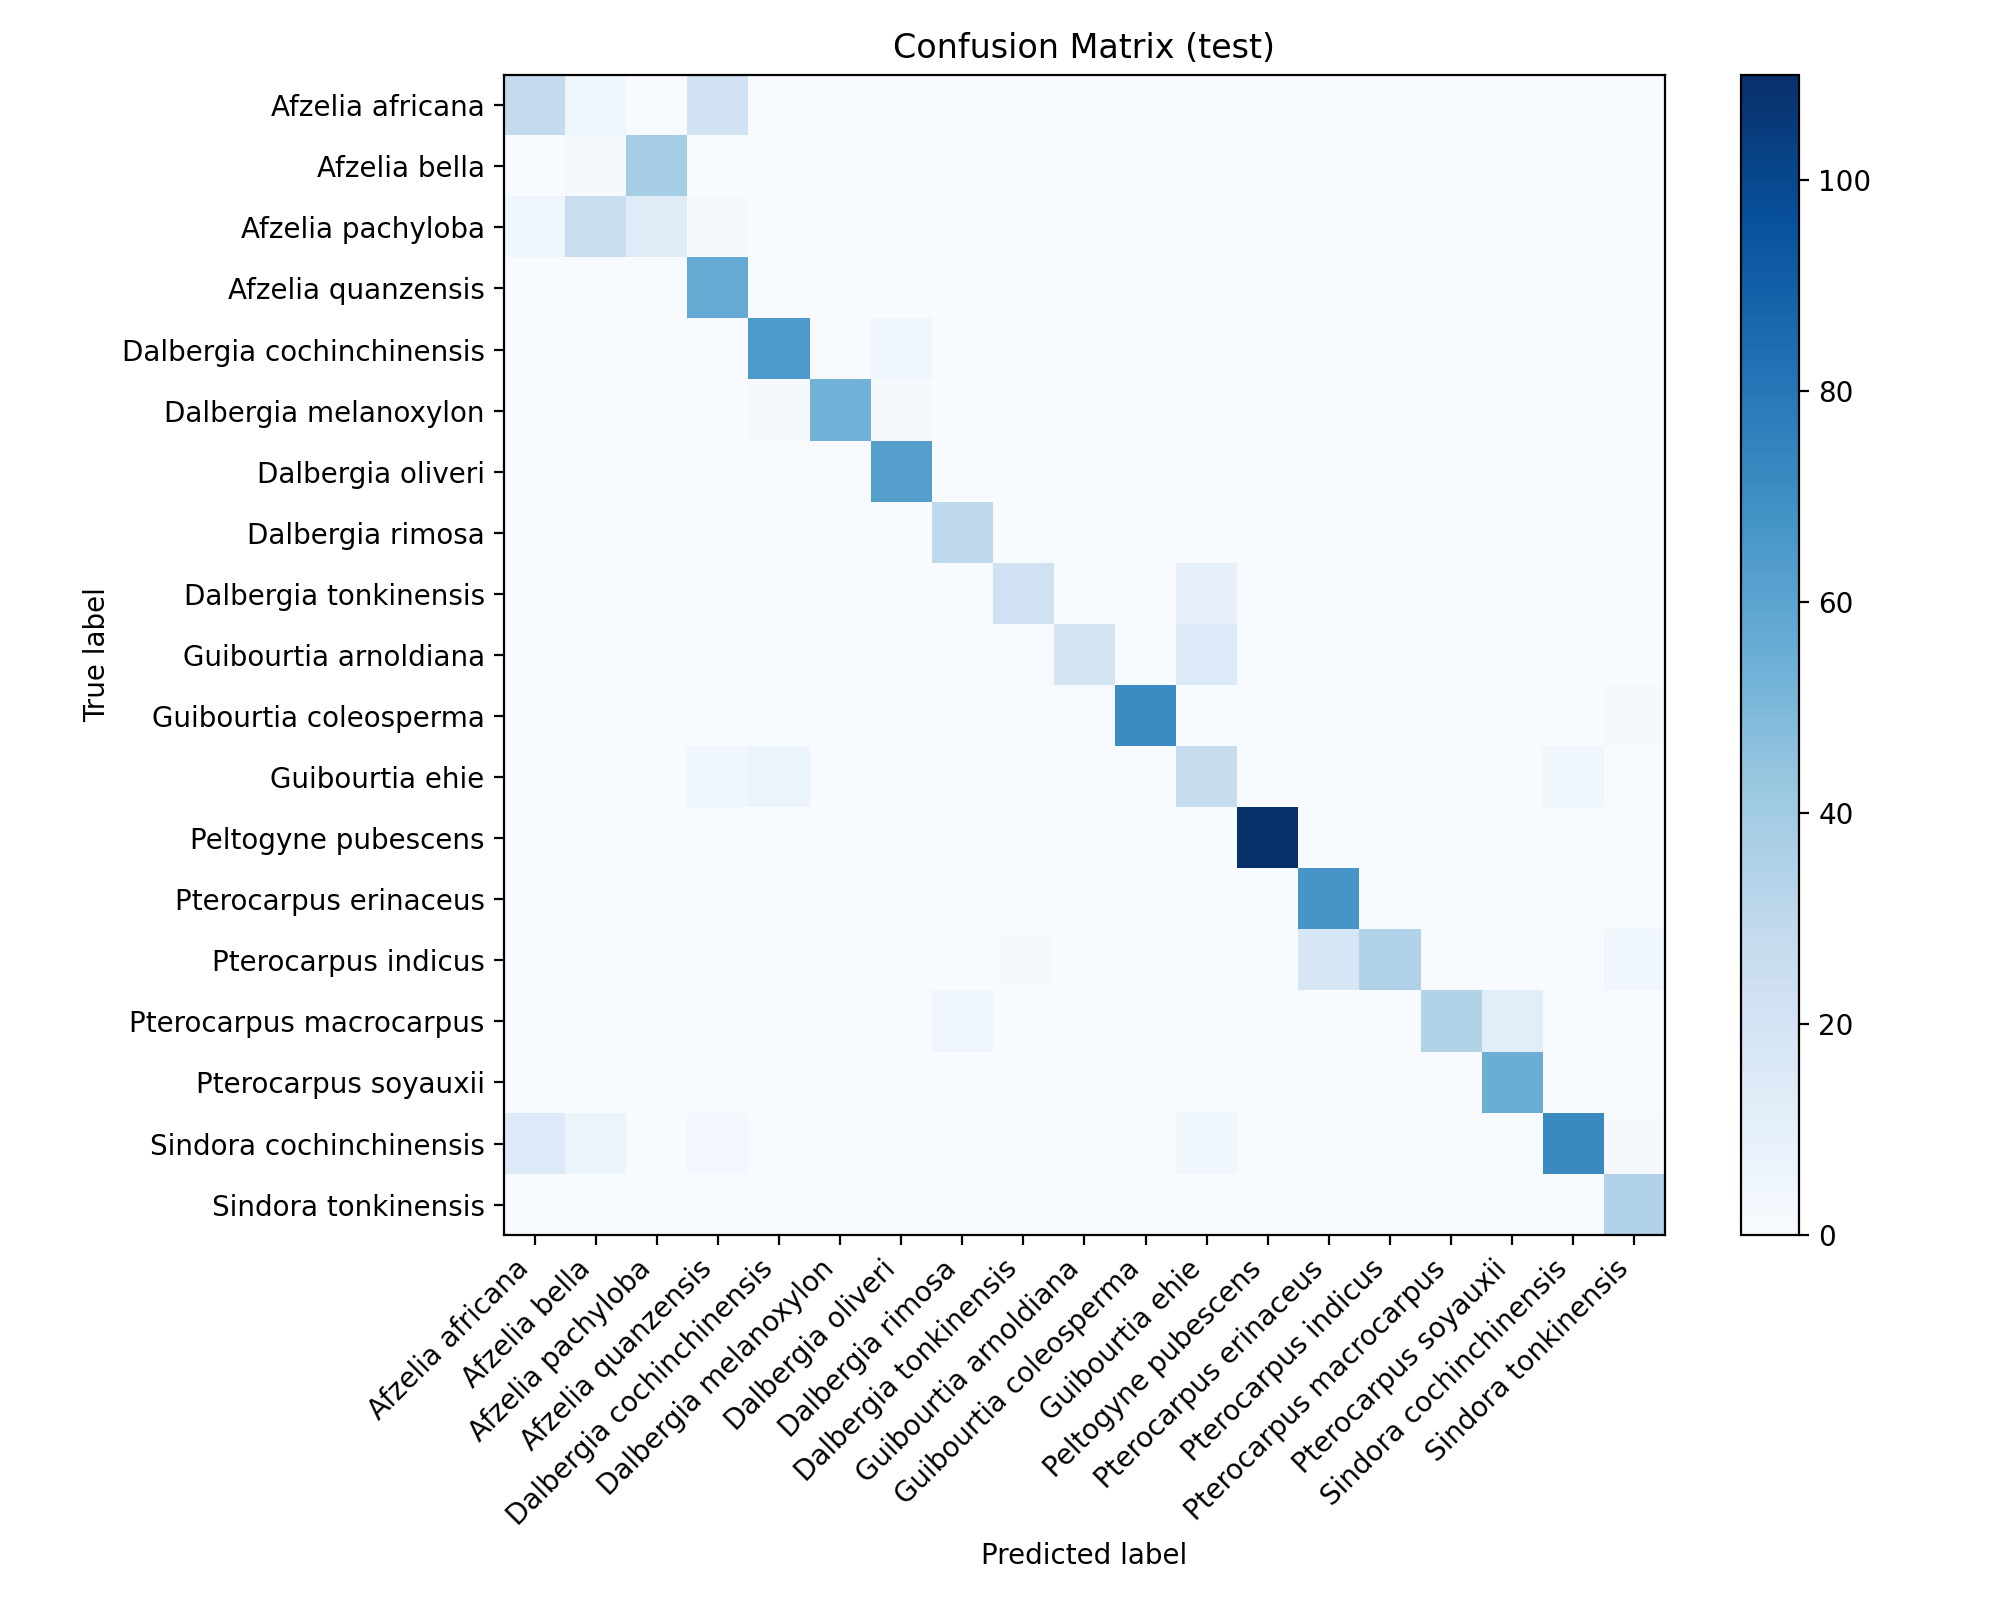
\includegraphics[width=\columnwidth]{fig/confusion_matrix_test.png}
\caption{Confusion matrix of the baseline model on the CEGS-Split test set.}
\label{fig:confusion_matrix}
\end{figure}

\subsection{Sensitivity to the Split Unit}
Bảng \ref{tab:split_ablation} so sánh KNN trên embedding Swin-Large đóng băng (frozen Swin-Large) giữa random image split và CEGS-Split. Random image split đạt KNN accuracy trung bình $0.9581$, trong khi CEGS-Split đạt $0.9087$; chênh lệch là $0.0494$ điểm tuyệt đối. Macro-F1 thay đổi từ $0.9493$ xuống $0.8858$. Vì feature extractor và bộ phân loại KNN được giữ nguyên, thí nghiệm cho thấy đơn vị split có thể thay đổi đáng kể kết quả evaluation.

\begin{table*}[htbp]
\centering
\caption{Sensitivity of KNN on frozen Swin-Large embeddings to the data split. Cosine similarity is reported as an inter-split image-level statistic.}
\label{tab:split_ablation}
\resizebox{\textwidth}{!}{%
\begin{tabular}{llccccccc}
\toprule
\textbf{Split} & \textbf{Seed} & \textbf{KNN Acc.} & \textbf{Macro-F1} & \textbf{Weighted-F1} & \textbf{Mean CosSim} & \textbf{Max CosSim} & \textbf{Train} & \textbf{Test} \\
\midrule
Random image & 42 & 0.9522 & 0.9343 & 0.9495 & 0.5678 & 0.9139 & 3900 & 1026 \\
Random image & 123 & 0.9429 & 0.9390 & 0.9426 & 0.5754 & 0.9173 & 3963 & 1015 \\
Random image & 456 & 0.9793 & 0.9745 & 0.9792 & 0.5758 & 0.9171 & 3895 & 1064 \\
CEGS-Split & 42 & 0.9087 & 0.8858 & 0.9062 & 0.5711 & 0.8999 & 4151 & 1041 \\
\midrule
Random image (mean) & --- & $0.9581 \pm 0.0155$ & $0.9493 \pm 0.0179$ & $0.9571 \pm 0.0159$ & $0.5730 \pm 0.0037$ & $0.9161 \pm 0.0015$ & --- & --- \\
CEGS-Split & --- & 0.9087 & 0.8858 & 0.9062 & 0.5711 & 0.8999 & --- & --- \\
\bottomrule
\end{tabular}%
}
\end{table*}

Độ tương đồng cosine cực đại (max cosine similarity) giảm từ $0.9161$ xuống $0.8999$ khi dùng CEGS-Split, còn mean cosine similarity thay đổi nhỏ. Đây là dấu hiệu nhất quán với việc random image split tạo ra một số cặp train--test gần nhau hơn; tuy nhiên các số cosine không tự chứng minh rằng một cặp ảnh có cùng nguồn. Kết luận về rò rỉ phải dựa trên giao của \texttt{specimen\_id} giữa các tập và kiểm tra manifest. Theo cách diễn giải thận trọng, kết quả trên chỉ xác lập rằng điểm số của cùng một pipeline nhạy với cách nhóm các ảnh thành đơn vị split.

CEGS-Split không được thiết kế để làm bài toán dễ hơn hoặc khó hơn một cách tùy ý. Nó xác định câu hỏi đánh giá khác: nhận diện một ảnh từ mẫu vật chưa xuất hiện trong quá trình training (held-out specimens). Do đó, chênh lệch $4.94$ điểm phần trăm không nên được gọi là mức đánh giá quá cao có thể khái quát cho mọi bộ dữ liệu; đây là mức khác biệt quan sát được trên S3, embedding và cấu hình KNN hiện tại.

\subsection{Implications for Representation Learning Benchmarks}
Kết quả cho thấy benchmark các loss functions chỉ có ý nghĩa khi split được khóa (frozen) trước khi thực hiện. Với cùng CEGS-Split, các phương pháp metric learning và self-supervised learning có thể được so sánh bằng retrieval, clustering và macro-F1. Khi công bố kết quả đầy đủ, mỗi phương pháp cần báo cáo seed, checkpoint selection rule, số specimen trong mỗi tập và độ biến thiên qua các lần chạy. Báo cáo một điểm số duy nhất trên random image split không đủ để tách biệt tác động của kiến trúc mạng khỏi tác động của cấu trúc split dữ liệu.

\subsection{Limitations}
Thứ nhất, kết quả CEGS-Split hiện dựa trên một split đã khóa; vì thế chưa thể suy ra khoảng tin cậy của chính protocol. Thứ hai, khả năng tổng quát hóa ngoài S3, đặc biệt sang thiết bị, điều kiện bề mặt hoặc nguồn mẫu khác, chưa được kiểm chứng bằng external test set. Thứ ba, độ tin cậy của split theo mẫu vật phụ thuộc trực tiếp vào độ đầy đủ của manifest. Những giới hạn này là động cơ để phát hành manifest phiên bản hóa, nhiều group-disjoint split và một tập test ngoài nguồn (external test set) trong các nghiên cứu tiếp theo.
